\begin{frame}{Quy trình các bước thu thập dữ liệu văn bản pháp luật}
\begin{figure}[H]
\centering
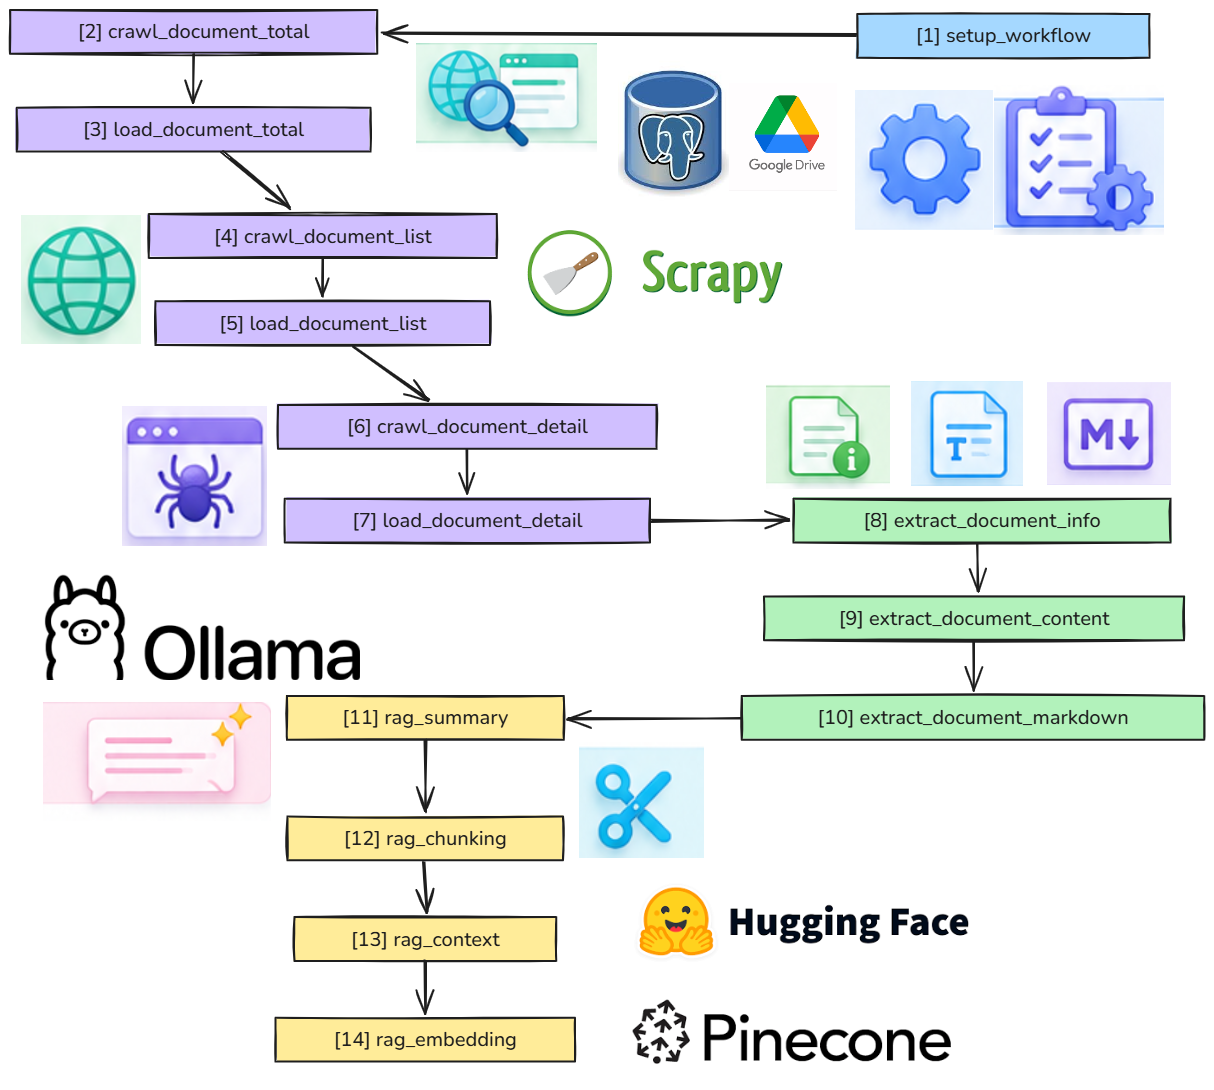
\includegraphics[height=0.55\textheight,width=0.9\textwidth,keepaspectratio]{pictures/step0.excalidraw.png}
\caption{Sơ đồ các bước thực hiện của quy trình cũ}
\end{figure}

\note{
Sơ đồ chi tiết các bước thực hiện trong quy trình cũ của đường ống dữ liệu văn bản pháp luật.
Quy trình được chia thành 3 giai đoạn: Khởi tạo luồng công việc (\texttt{step\_setup\_workflow}), thu thập tổng số lượng tài liệu (\texttt{step\_crawl\_document\_total}), tải nội dung chi tiết và cuối cùng là xử lý định dạng văn bản để chuẩn bị cho việc trích xuất thông tin.
}
\end{frame}
